\documentclass{standalone}
\usepackage{tikz}
\usepackage{amsmath}

\begin{document}

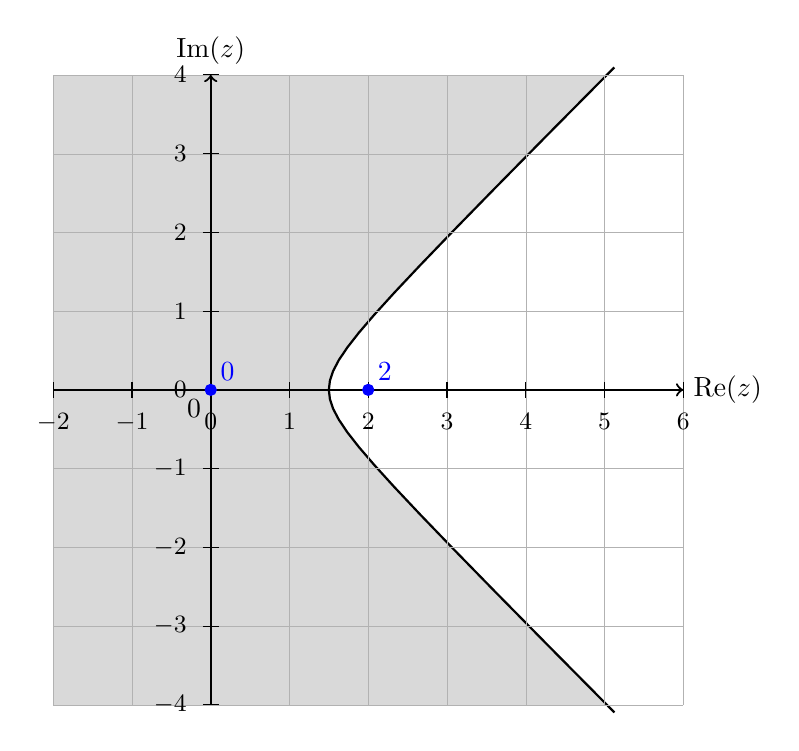
\begin{tikzpicture}
    
    % Center of the circle
    \def\xmin{-2}
    \def\xmax{6}
    \def\ymin{-4}
    \def\ymax{4}
    \def\dx{.5}
    \def\dy{.5}
    \def\xminb{\xmin-\dx}
    \def\xmaxb{\xmax+\dx}
    \def\yminb{\ymin-\dy}
    \def\ymaxb{\ymax+\dy}
    \def\xa{0.}
    \def\ya{0.}
    \def\xb{2.}
    \def\yb{0.}
    \def\a{0.5};
    \coordinate (fa) at (\xa, \ya);
    \coordinate (fb) at (\xb, \yb);
    \def\c{sqrt((\xa-\xb)^2+(\ya-\yb)^2)/2};
    \def\xc{0.5*(\xa+\xb)};
    \def\yc{0.5*(\ya+\yb)};
    \coordinate (center) at ({\xc}, {\yc});
    \def\b{sqrt(\c^2-\a^2)};
    \def\alpha{{atan2(\yb-\ya,\xb-\xa)}};

    % Fill outside region
    \begin{scope}
        % \clip (\xminb, \yminb) rectangle (\xmaxb, \ymaxb);
        \fill[gray!30] (\xmin, \ymin) rectangle (5, \ymax);
        % \fill[gray!30] (center) circle (3);
    \end{scope}
    
    \draw[thick, black, fill=white] plot[parametric, domain=-2.8:2.8] 
        ({\xc+\a*cosh(\x)}, {\yc+\b*sinh(\x)}); % Draw the parametric line
        

    % Draw grid
    \draw[step=1., gray!60, ultra thin] (\xmin, \ymin) grid (\xmax, \ymax); % Visible grid with lighter color
    
    % Axes
    \draw[->, thick] (\xmin, 0) -- (\xmax, 0) node[right] {$\text{Re}(z)$};
    \draw[->, thick] (0, \ymin) -- (0, \ymax) node[above] {$\text{Im}(z)$};

    % Axis ticks
    \foreach \x in {\xmin,..., \xmax}
        \draw (\x, -0.1) -- (\x, 0.1) node[below=8pt] {\small $\x$};
    \foreach \y in {\ymin,..., \ymax}
        \draw (-0.1, \y) -- (0.1, \y) node[left=8pt] {\small $\y$};

    % Labels for axes
    \node[below left] at (0, 0) {$0$};

    % Foci
    \filldraw[blue] (\xa, \ya) circle (2pt) node[above right] {$0$};
    \filldraw[blue] (\xb, \yb) circle (2pt) node[above right] {$2$};
    
\end{tikzpicture}

\end{document}
